\documentclass[a4paper,12pt]{article}

\usepackage{cmap} % ОБЯЗАТЕЛЬНО ПЕРВЫМ: исправляет поиск, выделение и копирование русского текста
\usepackage[utf8]{inputenc}
\usepackage[T2A]{fontenc}
\usepackage[russian]{babel}

% Векторные четкие шрифты (Times New Roman) и микротипографика
\usepackage{tempora}   % Качественный векторный шрифт (не будет пикселей и мыла)
\usepackage{microtype} % Идеальное сглаживание и межбуквенные интервалы

\usepackage{geometry}
\geometry{left=2.5cm, right=2cm, top=2cm, bottom=2cm}

\usepackage{array}
\usepackage{multirow}
\usepackage{graphicx}
\usepackage{float}
\usepackage{caption}
\usepackage{longtable}
\usepackage{amsmath}

\usepackage{pgfplots}
\pgfplotsset{compat=1.18}

\makeatletter
\renewcommand{\fnum@figure}{\normalsize Рисунок~\thefigure}
\makeatother

\captionsetup[figure]{
    justification=centering,
    font=normalsize,
    labelsep=endash,
    singlelinecheck=false
}

\captionsetup[table]{
    justification=centering,
    font=normalsize,
    labelsep=endash,
    singlelinecheck=false
}

\usepackage{titlesec}
\titleformat{\section}{\normalfont\large}{}{0pt}{}
\titleformat{\subsection}{\normalfont\large}{}{0pt}{}

\begin{document}

\thispagestyle{empty}

\textbf{
\begin{table}[h!]
\resizebox{\textwidth}{!}{%
\begin{tabular}{cc}
\footnotesize{Университет ИТМО}
&
\multirow{3}{*}{
    
\includegraphics[width=0.25\linewidth]{logo_ITMO.pdf}
}
\\
\footnotesize{Физико-технический мегафакультет} & \\
\footnotesize{Физический факультет} &
\end{tabular}%
}
\end{table}
}

\vspace{-0.5cm}

\begin{center}
\begin{tabular}{p{0.49\textwidth}p{0.49\textwidth}}

Группа: \textbf{Z3143} & К работе допущен \hrulefill \\

& \\

Студент: \textbf{Коровин Иван Вадимович}
& Работа выполнена: 05.09.2026 \\

& \\

Преподаватель: Смирнов А.В. & Отчет принят \hrulefill \\

\end{tabular}
\end{center}

\vspace{1cm}

\begin{center}

\huge{\textbf{Отчет по лабораторной работе № 1.01}} \\

\vspace{0.5cm}

\textbf{«Исследование распределения случайной величины»}

\end{center}

\section*{\hspace{30pt} Цель работы}

Исследование распределения случайной величины на примере
многократных измерений определённого интервала времени.

\section*{\hspace{30pt} Задачи, решаемые при выполнении работы}

\begin{enumerate}
    \item Провести многократные измерения определённого интервала времени.
    
    \item Построить гистограмму распределения результатов измерения.
    
    \item Вычислить среднее значение и дисперсию полученной выборки.
    
    \item Сравнить гистограмму с графиком функции Гаусса с такими же,
    как и у экспериментального распределения, средним значением и дисперсией.
\end{enumerate}

\newpage

% Страница 2
\section*{\hspace{30pt} 1. Схема установки}

\begin{figure}[H]
    \centering
    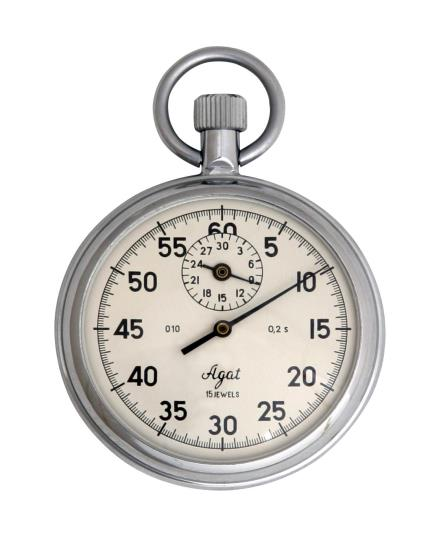
\includegraphics[width=0.35\textwidth]{Стрелочный секундомер.jpg}
    \caption{Стрелочный секундомер}
    \label{fig:analog-stopwatch}
\end{figure}

\begin{figure}[H]
    \centering
    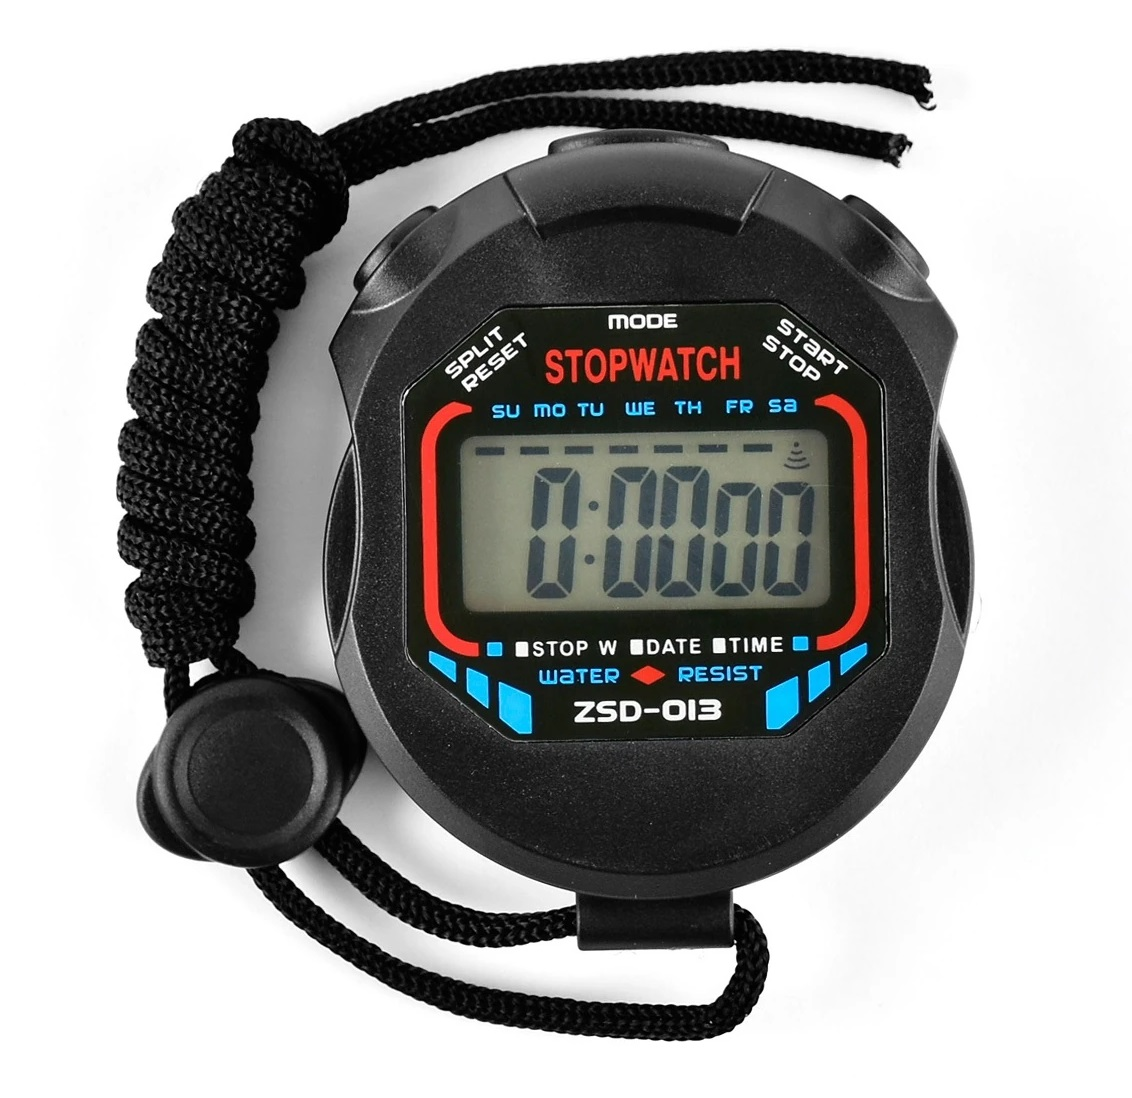
\includegraphics[width=0.35\textwidth]{Электронный секундомер.jpg}
    \caption{Цифровой секундомер}
    \label{fig:digital-stopwatch}
\end{figure}

\begin{figure}[H]
    \centering
    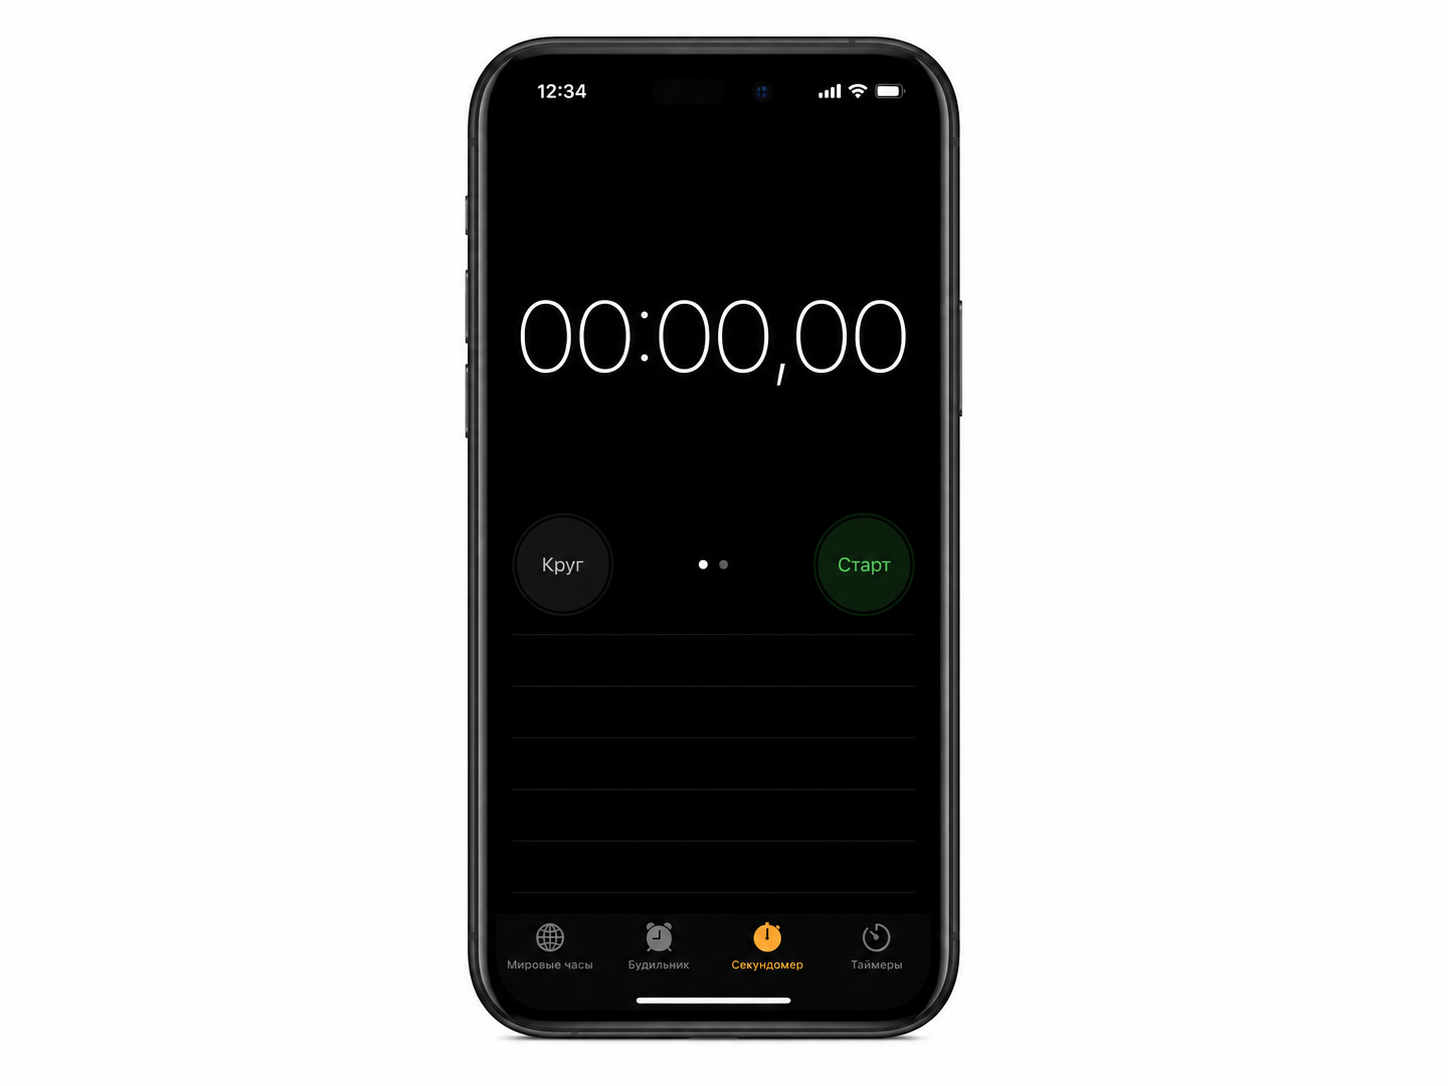
\includegraphics[width=0.55\textwidth]{Секундомер на телефоне.png}
    \caption{Секундомер мобильного устройства}
    \label{fig:mobile-device-stopwatch}
\end{figure}

\begin{table}[H]
    \centering
    \caption{Средства измерений}
    \label{tab:instruments}
    \begin{tabular}{|c|l|c|c|c|}
        \hline
        № & Наименование & Тип прибора & Диапазон, с & Погрешность, с \\
        \hline
        1 & Электронный секундомер  & Измерительный & 0-99 & 0{,}005 \\
        \hline
        2 & Секундомер мобильного устройства & Измерительный & 0-99 & 0{,}005 \\
        \hline
    \end{tabular}
\end{table}

\newpage

\section*{\hspace{30pt} 2. Рабочие формулы}

Количество проведённых измерений:
\begin{equation}
N=100,
\end{equation}
где $N$ --- количество измерений.

Среднее арифметическое значение результатов измерений определяется по формуле
\begin{equation}
\langle t\rangle_N =
\frac{1}{N}\sum_{i=1}^{N}t_i,
\end{equation}
где $t_i$ --- результат $i$-го измерения времени, $[t_i] = \text{с}$, $N$ --- количество измерений, $\langle t\rangle_N$ --- среднее значение измеряемой величины, $[\langle t\rangle_N] = \text{с}$.

Контроль правильности вычисления среднего значения:
\begin{equation}
\sum_{i=1}^{N}(t_i - \langle t\rangle_N) \approx 0,
\end{equation}
где $[t_i - \langle t\rangle_N] = \text{с}$.

Среднеквадратичное отклонение результатов измерений определяется по формуле
\begin{equation}
\sigma_N =
\sqrt{
\frac{1}{N-1}
\sum_{i=1}^{N}
\left(t_i-\langle t\rangle_N\right)^2
},
\end{equation}
где $\sigma_N$ --- среднеквадратичное отклонение результатов измерений, $[\sigma_N] = \text{с}$, $t_i$ --- результат $i$-го измерения, $\langle t\rangle_N$ --- среднее значение измеряемой величины, $N$ --- количество измерений.

Для построения гистограммы число интервалов выбирается близким к корню из количества измерений:
\begin{equation}
m\approx\sqrt{N},
\end{equation}
где $m$ --- количество интервалов гистограммы, $N$ --- количество измерений.

Плотность распределения для каждого интервала гистограммы определяется по формуле
\begin{equation}
\rho_i =
\frac{\Delta N_i}{N\Delta t},
\end{equation}
где $\rho_i$ --- плотность распределения в $i$-м интервале, $[\rho_i] = \text{с}^{-1}$, $\Delta N_i$ --- количество результатов измерений, попавших в $i$-й интервал, $N$ --- общее количество измерений, $\Delta t$ --- ширина интервала гистограммы, $[\Delta t] = \text{с}$.

Теоретическая плотность нормального распределения определяется по формуле
\begin{equation}
\rho(t) =
\frac{1}{\sigma\sqrt{2\pi}}
\exp\left(
-\frac{
\left(t-\langle t\rangle\right)^2
}{
2\sigma^2
}
\right),
\end{equation}
где $\rho(t)$ --- плотность распределения измеряемой величины, $[\rho(t)] = \text{с}^{-1}$, $t$ --- значение измеряемого времени, $[t] = \text{с}$, $\langle t\rangle$ --- среднее значение, $\sigma$ --- среднеквадратичное отклонение результатов измерений.

Максимальное значение плотности распределения определяется по формуле
\begin{equation}
\rho_{\max} =
\frac{1}{\sigma\sqrt{2\pi}},
\end{equation}
где $\rho_{\max}$ --- максимальное значение плотности распределения, $[\rho_{\max}] = \text{с}^{-1}$, $\sigma$ --- среднеквадратичное отклонение результатов измерений.

Среднеквадратичное отклонение среднего значения определяется по формуле
\begin{equation}
\sigma_{\langle t\rangle} =
\sqrt{
\frac{1}{N(N-1)}
\sum_{i=1}^{N}
\left(t_i-\langle t\rangle_N\right)^2
} = \frac{\sigma_N}{\sqrt{N}},
\end{equation}
где $\sigma_{\langle t\rangle}$ --- среднеквадратичное отклонение среднего значения, $[\sigma_{\langle t\rangle}] = \text{с}$, $t_i$ --- результат $i$-го измерения, $\langle t\rangle_N$ --- среднее значение, $N$ --- количество измерений.

Доверительный интервал для среднего значения определяется с помощью коэффициента Стьюдента:
\begin{equation}
\Delta t =
t_{\alpha,N}\sigma_{\langle t\rangle},
\qquad \alpha=0{,}95,
\end{equation}
где $\Delta t$ --- доверительная погрешность среднего значения, $[\Delta t] = \text{с}$, $t_{\alpha,N}$ --- коэффициент Стьюдента для доверительной вероятности $\alpha$ и числа измерений $N$, $\sigma_{\langle t\rangle}$ --- среднеквадратичное отклонение среднего значения, $\alpha$ --- доверительная вероятность.

Относительная погрешность измерения:
\begin{equation}
\varepsilon = \frac{\Delta t}{\langle t\rangle_N} \cdot 100\%.
\end{equation}

Итоговый результат измерения записывается в виде
\begin{equation}
t = \langle t\rangle_N \pm \Delta t, \qquad P = \alpha,
\end{equation}
где $t$ --- измеренное значение времени, $\langle t\rangle_N$ --- среднее значение результатов измерений, $\Delta t$ --- доверительная погрешность среднего значения.

\newpage

% Страница 3
\section*{\hspace{30pt} 3. Протокол измерений}

\begin{longtable}{|c|c|c|c|c|c|c|c|}
    \caption{Результаты прямых измерений}
    \label{tab:measurements} \\

    \hline
    № & $t_i$, с & $t_i-\langle t \rangle_N$, с & $(t_i-\langle t \rangle_N)^2$, с$^2$
    & № & $t_i$, с & $t_i- \langle t \rangle _N$, с & $(t_i- \langle t \rangle _N)^2$, с$^2$ \\
    \hline
    \endfirsthead

    \hline
    № & $t_i$, с & $t_i- \langle t \rangle _N$, с & $(t_i- \langle t \rangle _N)^2$, с$^2$
    & № & $t_i$, с & $t_i- \langle t \rangle _N$, с & $(t_i- \langle t \rangle _N)^2$, с$^2$ \\
    \hline
    \endhead

    1  & 4{,}81 & -0{,}133 & 0{,}017689 & 51  & 4{,}85 & -0{,}093 & 0{,}008649 \\ \hline
    2  & 5{,}09 & 0{,}147  & 0{,}021609 & 52  & 4{,}75 & -0{,}193 & 0{,}037249 \\ \hline
    3  & 5{,}06 & 0{,}117  & 0{,}013689 & 53  & 5{,}01 & 0{,}067  & 0{,}004489 \\ \hline
    4  & 4{,}69 & -0{,}253 & 0{,}064009 & 54  & 4{,}73 & -0{,}213 & 0{,}045369 \\ \hline
    5  & 4{,}91 & -0{,}033 & 0{,}001089 & 55  & 4{,}84 & -0{,}103 & 0{,}010609 \\ \hline
    6  & 5{,}06 & 0{,}117  & 0{,}013689 & 56  & 4{,}90 & -0{,}043 & 0{,}001849 \\ \hline
    7  & 4{,}81 & -0{,}133 & 0{,}017689 & 57  & 5{,}01 & 0{,}067  & 0{,}004489 \\ \hline
    8  & 5{,}15 & 0{,}207  & 0{,}042849 & 58  & 4{,}95 & 0{,}007  & 0{,}000049 \\ \hline
    9  & 4{,}88 & -0{,}063 & 0{,}003969 & 59  & 4{,}99 & 0{,}047  & 0{,}002209 \\ \hline
    10 & 4{,}88 & -0{,}063 & 0{,}003969 & 60  & 5{,}06 & 0{,}117  & 0{,}013689 \\ \hline
    11 & 4{,}94 & -0{,}003 & 0{,}000009 & 61  & 5{,}00 & 0{,}057  & 0{,}003249 \\ \hline
    12 & 5{,}00 & 0{,}057  & 0{,}003249 & 62  & 4{,}88 & -0{,}063 & 0{,}003969 \\ \hline
    13 & 5{,}03 & 0{,}087  & 0{,}007569 & 63  & 5{,}00 & 0{,}057  & 0{,}003249 \\ \hline
    14 & 4{,}75 & -0{,}193 & 0{,}037249 & 64  & 4{,}98 & 0{,}037  & 0{,}001369 \\ \hline
    15 & 5{,}06 & 0{,}117  & 0{,}013689 & 65  & 4{,}66 & -0{,}283 & 0{,}080089 \\ \hline
    16 & 4{,}84 & -0{,}103 & 0{,}010609 & 66  & 4{,}96 & 0{,}017  & 0{,}000289 \\ \hline
    17 & 4{,}75 & -0{,}193 & 0{,}037249 & 67  & 4{,}93 & -0{,}013 & 0{,}000169 \\ \hline
    18 & 4{,}91 & -0{,}033 & 0{,}001089 & 68  & 4{,}99 & 0{,}047  & 0{,}002209 \\ \hline
    19 & 4{,}87 & -0{,}073 & 0{,}005329 & 69  & 4{,}96 & 0{,}017  & 0{,}000289 \\ \hline
    20 & 4{,}97 & 0{,}027  & 0{,}000729 & 70  & 4{,}76 & -0{,}183 & 0{,}033489 \\ \hline
    21 & 4{,}85 & -0{,}093 & 0{,}008649 & 71  & 4{,}80 & -0{,}143 & 0{,}020449 \\ \hline
    22 & 4{,}84 & -0{,}103 & 0{,}010609 & 72  & 5{,}09 & 0{,}147  & 0{,}021609 \\ \hline
    23 & 5{,}06 & 0{,}117  & 0{,}013689 & 73  & 4{,}88 & -0{,}063 & 0{,}003969 \\ \hline
    24 & 4{,}97 & 0{,}027  & 0{,}000729 & 74  & 5{,}00 & 0{,}057  & 0{,}003249 \\ \hline
    25 & 4{,}94 & -0{,}003 & 0{,}000009 & 75  & 4{,}89 & -0{,}053 & 0{,}002809 \\ \hline
    26 & 4{,}85 & -0{,}093 & 0{,}008649 & 76  & 5{,}01 & 0{,}067  & 0{,}004489 \\ \hline
    27 & 5{,}00 & 0{,}057  & 0{,}003249 & 77  & 4{,}86 & -0{,}083 & 0{,}006889 \\ \hline
    28 & 4{,}90 & -0{,}043 & 0{,}001849 & 78  & 4{,}86 & -0{,}083 & 0{,}006889 \\ \hline
    29 & 5{,}12 & 0{,}177  & 0{,}031329 & 79  & 4{,}91 & -0{,}033 & 0{,}001089 \\ \hline
    30 & 5{,}16 & 0{,}217  & 0{,}047089 & 80  & 4{,}93 & -0{,}013 & 0{,}000169 \\ \hline
    31 & 5{,}07 & 0{,}127  & 0{,}016129 & 81  & 4{,}83 & -0{,}113 & 0{,}012769 \\ \hline
    32 & 4{,}87 & -0{,}073 & 0{,}005329 & 82  & 5{,}10 & 0{,}157  & 0{,}024649 \\ \hline
    33 & 5{,}03 & 0{,}087  & 0{,}007569 & 83  & 4{,}90 & -0{,}043 & 0{,}001849 \\ \hline
    34 & 5{,}06 & 0{,}117  & 0{,}013689 & 84  & 5{,}18 & 0{,}237  & 0{,}056169 \\ \hline
    35 & 4{,}69 & -0{,}253 & 0{,}064009 & 85  & 4{,}80 & -0{,}143 & 0{,}020449 \\ \hline
    36 & 5{,}03 & 0{,}087  & 0{,}007569 & 86  & 4{,}88 & -0{,}063 & 0{,}003969 \\ \hline
    37 & 4{,}93 & -0{,}013 & 0{,}000169 & 87  & 5{,}03 & 0{,}087  & 0{,}007569 \\ \hline
    38 & 4{,}85 & -0{,}093 & 0{,}008649 & 88  & 4{,}96 & 0{,}017  & 0{,}000289 \\ \hline
    39 & 5{,}09 & 0{,}147  & 0{,}021609 & 89  & 4{,}84 & -0{,}103 & 0{,}010609 \\ \hline
    40 & 5{,}09 & 0{,}147  & 0{,}021609 & 90  & 4{,}98 & 0{,}037  & 0{,}001369 \\ \hline
    41 & 5{,}06 & 0{,}117  & 0{,}013689 & 91  & 5{,}00 & 0{,}057  & 0{,}003249 \\ \hline
    42 & 5{,}06 & 0{,}117  & 0{,}013689 & 92  & 4{,}93 & -0{,}013 & 0{,}000169 \\ \hline
    43 & 4{,}90 & -0{,}043 & 0{,}001849 & 93  & 4{,}96 & 0{,}017  & 0{,}000289 \\ \hline
    44 & 4{,}84 & -0{,}103 & 0{,}010609 & 94  & 4{,}83 & -0{,}113 & 0{,}012769 \\ \hline
    45 & 5{,}03 & 0{,}087  & 0{,}007569 & 95  & 5{,}03 & 0{,}087  & 0{,}007569 \\ \hline
    46 & 5{,}00 & 0{,}057  & 0{,}003249 & 96  & 5{,}03 & 0{,}087  & 0{,}007569 \\ \hline
    47 & 5{,}10 & 0{,}157  & 0{,}024649 & 97  & 4{,}93 & -0{,}013 & 0{,}000169 \\ \hline
    48 & 5{,}06 & 0{,}117  & 0{,}013689 & 98  & 5{,}11 & 0{,}167  & 0{,}027889 \\ \hline
    49 & 5{,}03 & 0{,}087  & 0{,}007569 & 99  & 4{,}91 & -0{,}033 & 0{,}001089 \\ \hline
    50 & 4{,}78 & -0{,}163 & 0{,}026569 & 100 & 4{,}91 & -0{,}033 & 0{,}001089 \\ \hline

    \multicolumn{8}{|c|}{$\langle t \rangle _N = \text{4{,}943 с};\quad \sum_{i=1}^{100} (t_i - \langle t \rangle _N) = 0{,}000\text{ с};\quad \sigma_N = \text{0{,}113 с};\quad \rho_{\max} = \text{3{,}534 c}^{-1}$} \\
    \hline

\end{longtable}

Минимальное и максимальное значения времени: $t_{\min} = \text{4{,}66 c}$, $t_{\max} = \text{5{,}18 c}$.

\begin{figure}[H]
    \centering
    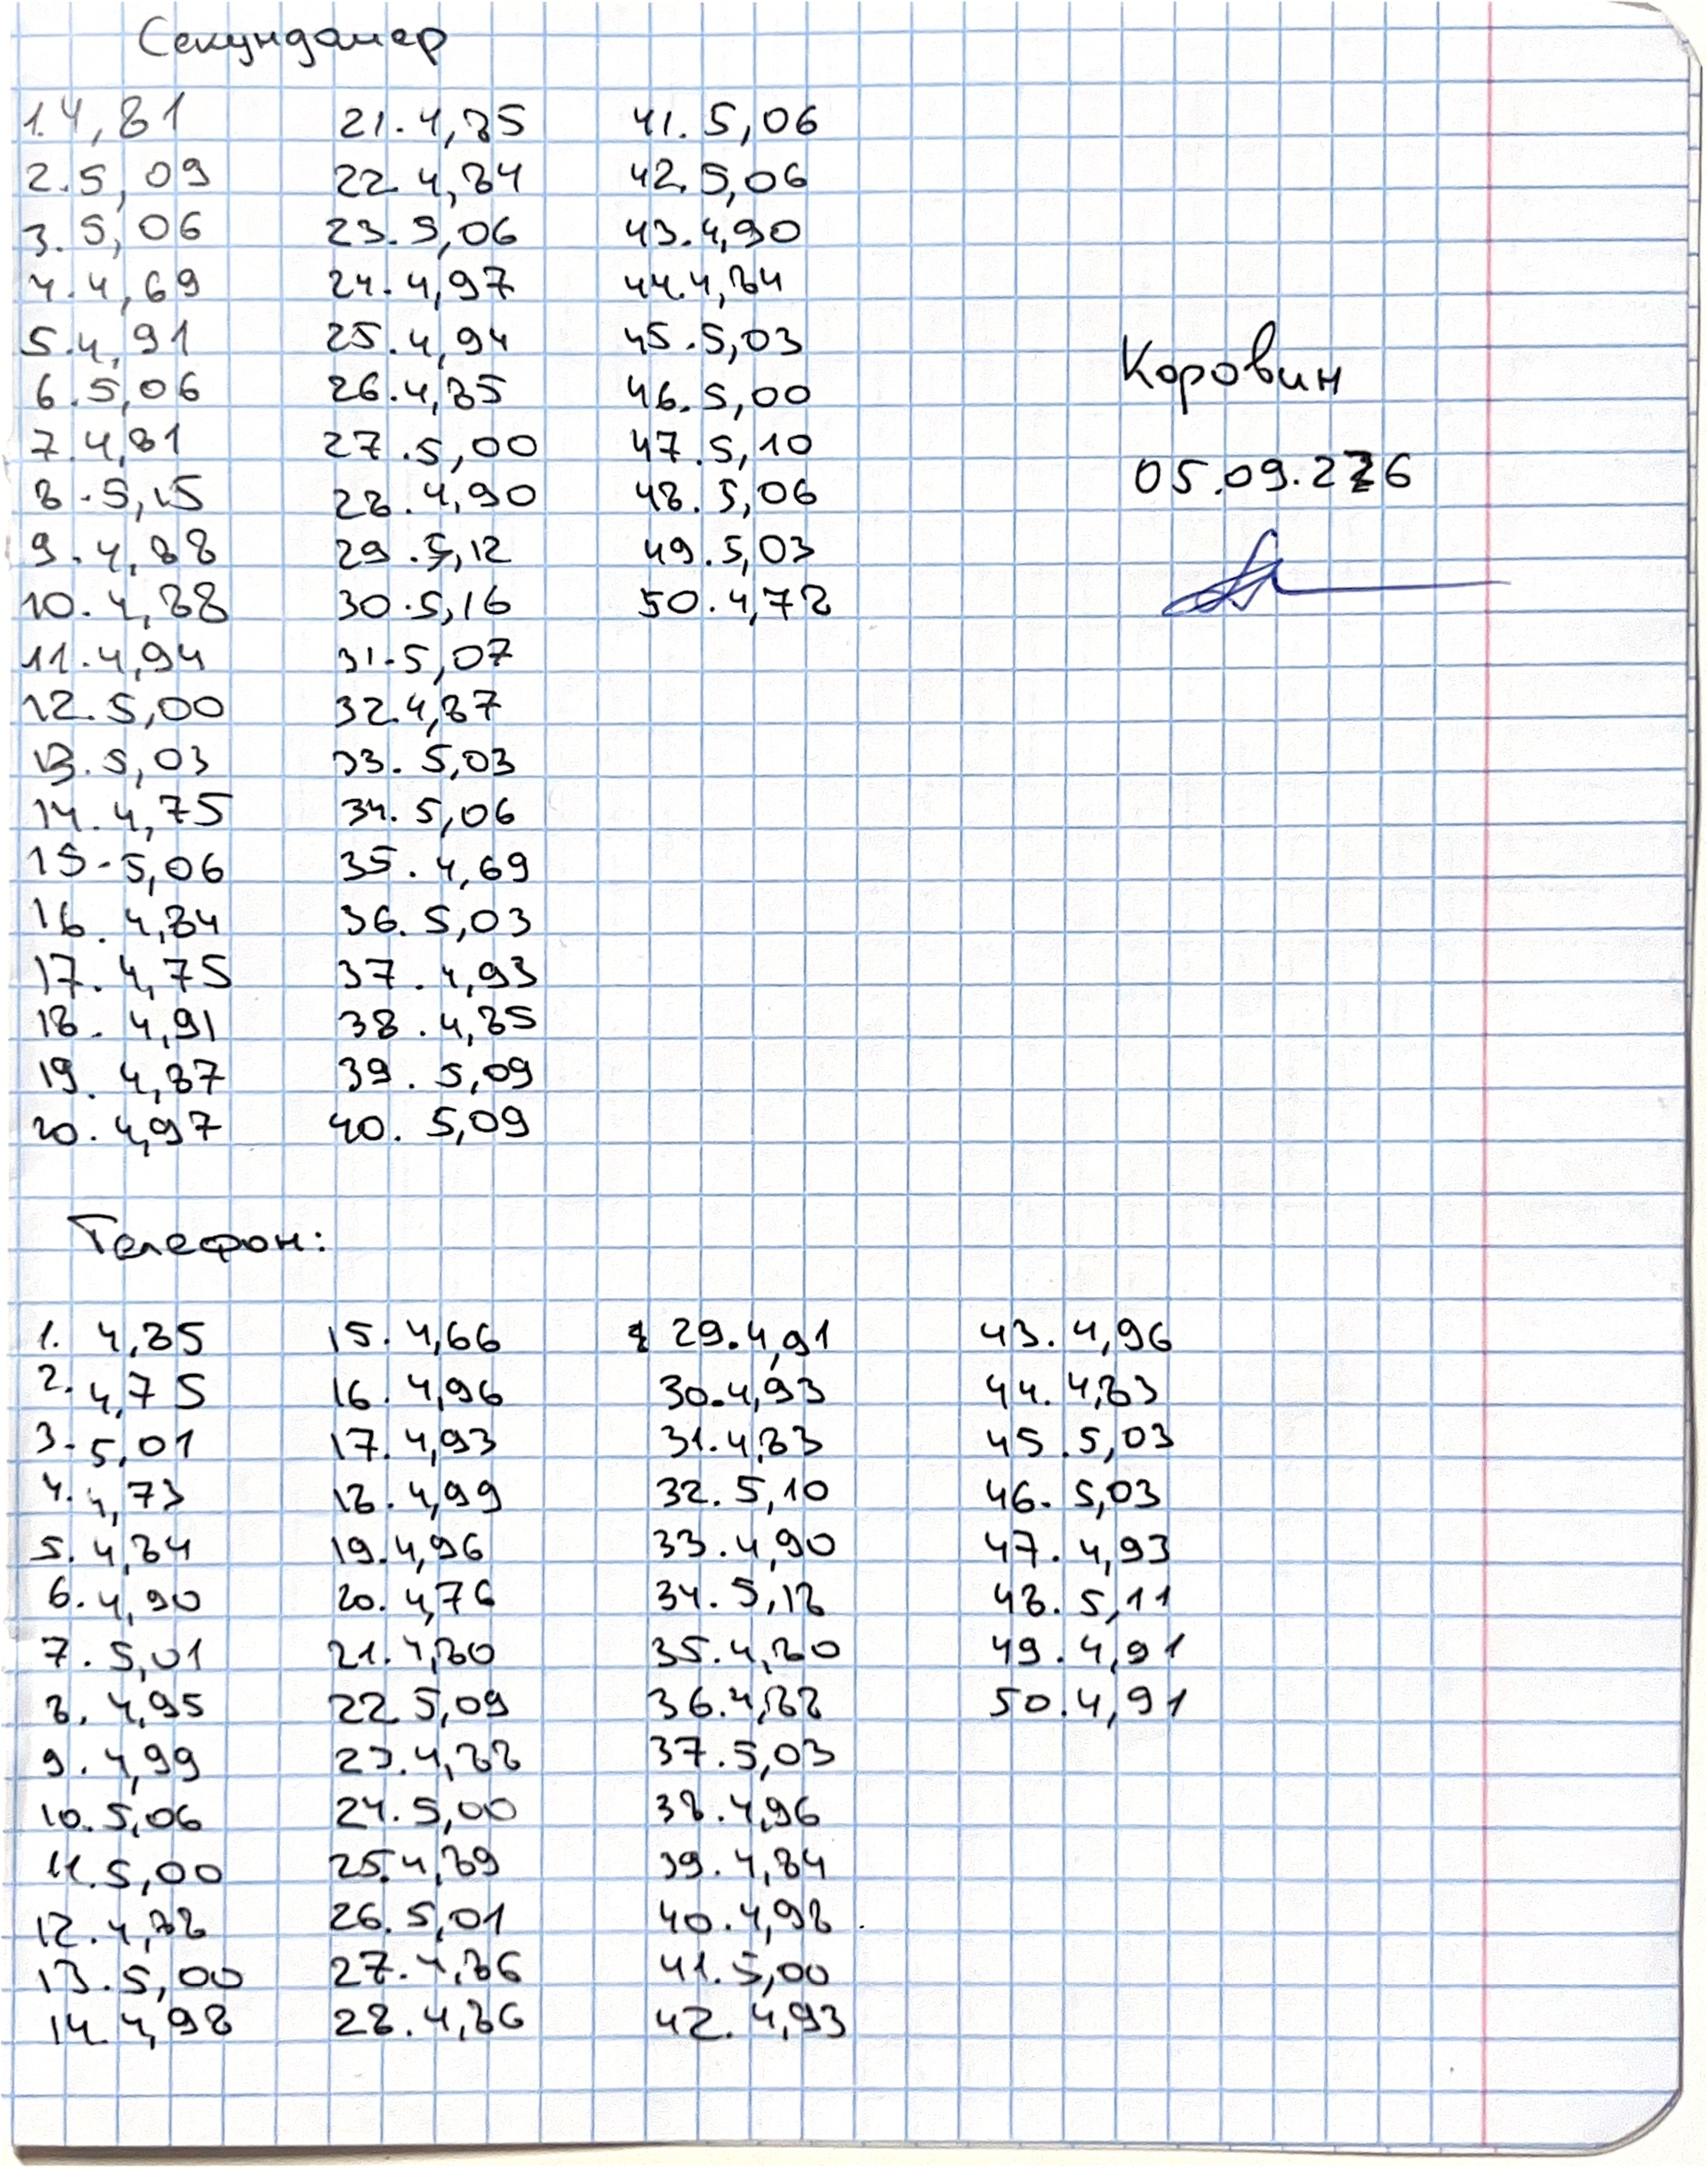
\includegraphics[width=0.75\textwidth]{1-01-izmerenia.pdf} 
    \caption{Подтверждённые измерения}
    \label{fig:confirmed-measurements}
\end{figure}

\newpage

% Страница 4
\section*{\hspace{30pt} 4. Обработка результатов измерений}

\begin{table}[H]
    \centering
    \caption{Данные для построения диаграммы}
    \label{tab:data-for-building-the-chart}
    \begin{tabular}{|c|c|c|c|c|}
        \hline
        Границы интервалов, с
        & $\Delta N$
        & $\frac{\Delta N}{N\Delta t}$, $\text{с}^{-1}$
        & $t$, с
        & $\rho$, $\text{с}^{-1}$ \\ \hline

        4{,}660 & \multirow{2}{*}{3}
        & \multirow{2}{*}{0{,}577}
        & \multirow{2}{*}{4{,}686}
        & \multirow{2}{*}{0{,}265} \\ \cline{1-1}
        4{,}712 & & & & \\ \hline

        4{,}712 & \multirow{2}{*}{5}
        & \multirow{2}{*}{0{,}962}
        & \multirow{2}{*}{4{,}738}
        & \multirow{2}{*}{0{,}680} \\ \cline{1-1}
        4{,}764 & & & & \\ \hline

        4{,}764 & \multirow{2}{*}{5}
        & \multirow{2}{*}{0{,}962}
        & \multirow{2}{*}{4{,}790}
        & \multirow{2}{*}{1{,}411} \\ \cline{1-1}
        4{,}816 & & & & \\ \hline

        4{,}816 & \multirow{2}{*}{13}
        & \multirow{2}{*}{2{,}500}
        & \multirow{2}{*}{4{,}842}
        & \multirow{2}{*}{2{,}368} \\ \cline{1-1}
        4{,}868 & & & & \\ \hline

        4{,}868 & \multirow{2}{*}{17}
        & \multirow{2}{*}{3{,}269}
        & \multirow{2}{*}{4{,}894}
        & \multirow{2}{*}{3{,}215} \\ \cline{1-1}
        4{,}920 & & & & \\ \hline

        4{,}920 & \multirow{2}{*}{14}
        & \multirow{2}{*}{2{,}692}
        & \multirow{2}{*}{4{,}946}
        & \multirow{2}{*}{3{,}531} \\ \cline{1-1}
        4{,}972 & & & & \\ \hline

        4{,}972 & \multirow{2}{*}{14}
        & \multirow{2}{*}{2{,}692}
        & \multirow{2}{*}{4{,}998}
        & \multirow{2}{*}{3{,}138} \\ \cline{1-1}
        5{,}024 & & & & \\ \hline

        5{,}024 & \multirow{2}{*}{18}
        & \multirow{2}{*}{3{,}462}
        & \multirow{2}{*}{5{,}050}
        & \multirow{2}{*}{2{,}255} \\ \cline{1-1}
        5{,}076 & & & & \\ \hline

        5{,}076 & \multirow{2}{*}{8}
        & \multirow{2}{*}{1{,}538}
        & \multirow{2}{*}{5{,}102}
        & \multirow{2}{*}{1{,}311} \\ \cline{1-1}
        5{,}128 & & & & \\ \hline

        5{,}128 & \multirow{2}{*}{3}
        & \multirow{2}{*}{0{,}577}
        & \multirow{2}{*}{5{,}154}
        & \multirow{2}{*}{0{,}617} \\ \cline{1-1}
        5{,}180 & & & & \\ \hline

    \end{tabular}
\end{table}

\begin{table}[H]
    \centering
    \caption{Стандартные доверительные интервалы}
    \label{tab:standart-intervals}
    \begin{tabular}{|l|c|c|c|c|c|}
        \hline
        \multirow{2}{*}{Интервал} & \multicolumn{2}{c|}{Интервал, с}
        & \multirow{2}{*}{$\Delta N$}
        & \multirow{2}{*}{$\dfrac{\Delta N}{N}$}
        & \multirow{2}{*}{$P$} \\
        \cline{2-3}
        & От & До & & & \\
        \hline
        $\langle t\rangle_N \pm \sigma_N$
        & 4{,}830 & 5{,}056 & 66 & 0{,}66 & 0{,}683\\
        \hline
        $\langle t\rangle_N \pm 2\sigma_N$
        & 4{,}717 & 5{,}169 & 96 & 0{,}96 & 0{,}954\\
        \hline
        $\langle t\rangle_N \pm 3\sigma_N$
        & 4{,}604 & 5{,}282 & 100 & 1{,}00 & 0{,}997\\
        \hline
    \end{tabular}
\end{table}

Среднеквадратичное отклонение среднего значения:
\begin{equation}
\sigma_{\langle t\rangle} = \sqrt{\frac{1}{N(N-1)} \sum_{i=1}^{N} (t_i - \langle t\rangle_N)^2} = \frac{\sigma_N}{\sqrt{N}} = \frac{0{,}113}{\sqrt{100}} = 0{,}0113\text{ с}.
\end{equation}

Коэффициент Стьюдента для $N = 100$ и доверительной вероятности $\alpha = 0{,}95$:
\begin{equation}
t_{\alpha, N} \approx 1{,}98.
\end{equation}

Доверительный интервал:
\begin{equation}
\Delta t = t_{\alpha, N} \cdot \sigma_{\langle t\rangle} = 1{,}98 \cdot 0{,}0113\text{ с} = 0{,}0224\text{ с} \approx 0{,}022\text{ с}.
\end{equation}

Относительная погрешность:
\begin{equation}
\varepsilon = \frac{\Delta t}{\langle t\rangle_N} \cdot 100\% = \frac{0{,}0224}{4{,}943} \cdot 100\% \approx 0{,}45\%.
\end{equation}

\newpage

\begin{figure}[H]
    \centering
    \begin{tikzpicture}
        \begin{axis}[
            ybar interval,
            width=14cm,
            height=8cm,
            xlabel={$t$, с},
            ylabel={$\frac{\Delta N}{N\Delta t}$, с$^{-1}$},
            xmin=4.66,
            xmax=5.18,
            ymin=0,
            xtick={4.66,4.712,4.764,4.816,4.868,4.92,4.972,5.024,5.076,5.128,5.18},
            xticklabel style={rotate=45, anchor=east},
            ymajorgrids=true,
        ]
            \addplot coordinates {
                (4.660, 0.577)
                (4.712, 0.962)
                (4.764, 0.962)
                (4.816, 2.500)
                (4.868, 3.269)
                (4.920, 2.692)
                (4.972, 2.692)
                (5.024, 3.462)
                (5.076, 1.538)
                (5.128, 0.577)
                (5.180, 0)
            };

            % Экспериментальные значения rho(t)
            \addplot[
                only marks,
                mark=*,
                mark size=2pt,
                thick
            ] coordinates {
                (4.686, 0.265120849)
                (4.738, 0.680016356)
                (4.790, 1.410940115)
                (4.842, 2.368162769)
                (4.894, 3.215350061)
                (4.946, 3.531496019)
                (4.998, 3.137638644)
                (5.050, 2.255074400)
                (5.102, 1.311090196)
                (5.154, 0.616620573)
            };

            % Теоретическая функция Гаусса
            \addplot[
                domain=4.660:5.180,
                samples=200,
                smooth,
                thick
            ] {
                1/(0.112927079*sqrt(2*pi))
                * exp(-(x-4.943)^2/(2*0.112927079^2))
            };

            % Подпись функции
            \draw[
                ->,
                >=stealth,
                thick
            ]
            (axis cs:4.75,3.30)
            -- (axis cs:4.86,2.83)
            node[pos=0, above left] {$\rho(t)$};

        \end{axis}
    \end{tikzpicture}
    \caption{Гистограмма распределения измеренных значений времени и функция Гаусса}
    \label{fig:histogram}
\end{figure}

\section*{\hspace{30pt} 5. Окончательные результаты}

В ходе обработки 100 измерений интервала времени ($T = 5\text{ с}$) получены следующие результаты:
\begin{itemize}
    \item Количество измерений: $N = 100$
    \item Среднее арифметическое значение: $\langle t\rangle_N = 4{,}943\text{ с}$
    \item Выборочное среднеквадратичное отклонение: $\sigma_N = 0{,}113\text{ с}$
    \item Выборочная дисперсия: $D_N = \sigma_N^2 = 0{,}0128\text{ с}^2$
    \item Максимальная плотность вероятности: $\rho_{\max} = 3{,}534\text{ с}^{-1}$
    \item Среднеквадратичное отклонение среднего: $\sigma_{\langle t\rangle} = 0{,}011\text{ с}$
    \item Коэффициент Стьюдента ($\alpha = 0{,}95$): $t_{\alpha, N} \approx 1{,}98$
    \item Доверительная погрешность: $\Delta t = 0{,}022\text{ с}$
    \item Относительная погрешность: $\varepsilon = 0{,}45\%$
\end{itemize}

\vspace{0.3cm}
\textbf{Итоговый результат измерения:}
\begin{equation*}
    t = (4{,}943 \pm 0{,}022)\text{ с}, \quad \alpha = 0{,}95, \quad \varepsilon = 0{,}45\%.
\end{equation*}

\newpage

% Страница 5
\section*{\hspace{30pt} 6. Выводы и анализ результатов работы}

\begin{enumerate}
    \item В ходе работы было выполнено $N = 100$ измерений заданного интервала времени $T = 5\text{ с}$. По этим данным построена гистограмма, поверх которой наложен график теоретического распределения Гаусса. Рассчитанные параметры распределения: среднее время $\langle t\rangle_N = 4{,}943\text{ с}$, стандартное отклонение $\sigma_N = 0{,}113\text{ с}$.
    
    \item Проверка на соответствие правилу (таблица~\ref{tab:standart-intervals}) показала следующие результаты:
    \begin{itemize}
        \item в интервал $\langle t\rangle_N \pm \sigma_N$ входит $66\%$ значений (теоретическое ожидание — $68{,}3\%$);
        \item в интервал $\langle t\rangle_N \pm 2\sigma_N$ входит $96\%$ значений (теоретическое ожидание — $95{,}4\%$);
        \item в интервал $\langle t\rangle_N \pm 3\sigma_N$ входит $100\%$ измерений (теоретическое ожидание — $99{,}7\%$).
    \end{itemize}
    
    \item Как видно из полученных долей, экспериментальные данные достаточно хорошо описываются нормальным распределением. Небольшие расхождения с теорией и лёгкая асимметрия гистограммы вполне ожидаемы. В первую очередь они связаны с ограниченным объёмом выборки (всего 100 измерений), а также с человеческим фактором — естественными колебаниями времени реакции при запуске и остановке секундомера.
    
    \item Относительная погрешность серии измерений составила $\varepsilon = 0{,}45\%$. Это говорит о том, что случайные ошибки в ходе эксперимента были невелики, а итоговый результат получился весьма точным.
\end{enumerate}

\vspace{1cm}

\section*{\hspace{30pt} 7. Приложение}

Расчёты и первичная обработка данных проводились в Microsoft Excel. Построение гистограммы и графика распределения Гаусса выполнено с помощью пакета \texttt{pgfplots} в \LaTeX.
\end{document}